\chapter{Results \& Analysis}
\label{ch:res}

Note, refer to \hyperlink{appendixa}{Appendix A} for all CFX results.

%-----------------------------------------------------------------------------------------------------------------
\section{Convergence}
\label{sec:convg}

$i_{ref}=39$ $i_1=36$ $i_2=44$

Reference model convergence Figure~\ref{fig:ref_convg}, Model 1 convergence Figure~\ref{fig:mod1_convg}, Model 2 convergence Figure~\ref{fig:mod2_convg}

\begin{figure}[H]
	\centering
	\includegraphics[width=0.5\textwidth]{ref/convergence}
	\caption{Reference model convergence.}
	\label{fig:ref_convg}
\end{figure}

\begin{figure}[H]
	\centering
	\includegraphics[width=0.5\textwidth]{model1/convergence}
	\caption{Model 1 convergence.}
	\label{fig:mod1_convg}
\end{figure}

\begin{figure}[H]
	\centering
	\includegraphics[width=0.5\textwidth]{model2/convergence}
	\caption{Model 2 convergence.}
	\label{fig:mod2_convg}
\end{figure}

%\begin{figure}[H]
%    \centering
%    \begin{subfigure}[b]{0.45\textwidth}
%        \includegraphics[width=\textwidth]{ref/convergence}
%        \caption{}
%        \label{fig:ref_convg}
%    \end{subfigure}%
%    ~% add a small space
%    \\% change line
%    \begin{subfigure}[b]{0.45\textwidth}
%        \includegraphics[width=\textwidth]{model1/convergence}
%        \caption{}
%        \label{fig:mod1_convg}
%    \end{subfigure}%
%   ~% add a small space
%    \\% change line
%    \begin{subfigure}[b]{0.45\textwidth}
%        \includegraphics[width=\textwidth]{model2/convergence}
%        \caption{}
%        \label{fig:mod2_convg}
%    \end{subfigure}%
%    \caption{Convergence}
%    \label{fig:convergence}
%\end{figure}
%

%-----------------------------------------------------------------------------------------------------------------
\section{Validation}
\label{sec:err}
Validation of the reference model is completed by comparing experimental data from \cite{art}. Velocity and turbulent kinetic energy data at $X^*=-0.87, 0, 1.6, 2.5, 4, 9$ are compared in the following plots.\\

Both simulated and experimental velocity $u$ profiles at various $X^*$ are shown below in Figure~\ref{fig:exp_ref_u} \cite{matlab}.
\begin{figure}[H]
	\centering
	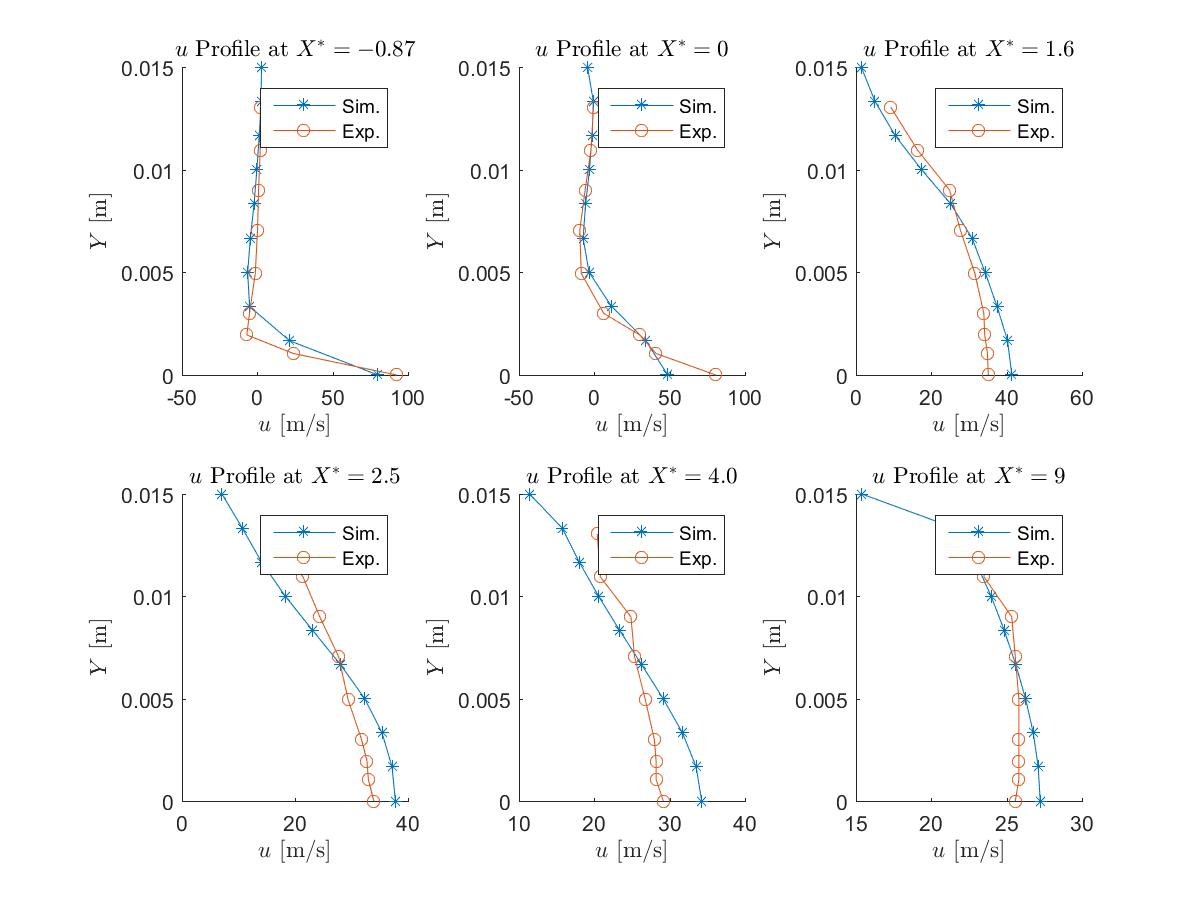
\includegraphics[scale=0.35]{matlab/exp_ref_u}
	\caption{Comparison of experimental and simulated $u$ profiles at various $X^*$.}
	\label{fig:exp_ref_u}
\end{figure}

Comments\\

Both simulated and experimental velocity $v$ profiles at various $X^*$ are shown below in Figure~\ref{fig:exp_ref_v}.
\begin{figure}[H]
	\centering
	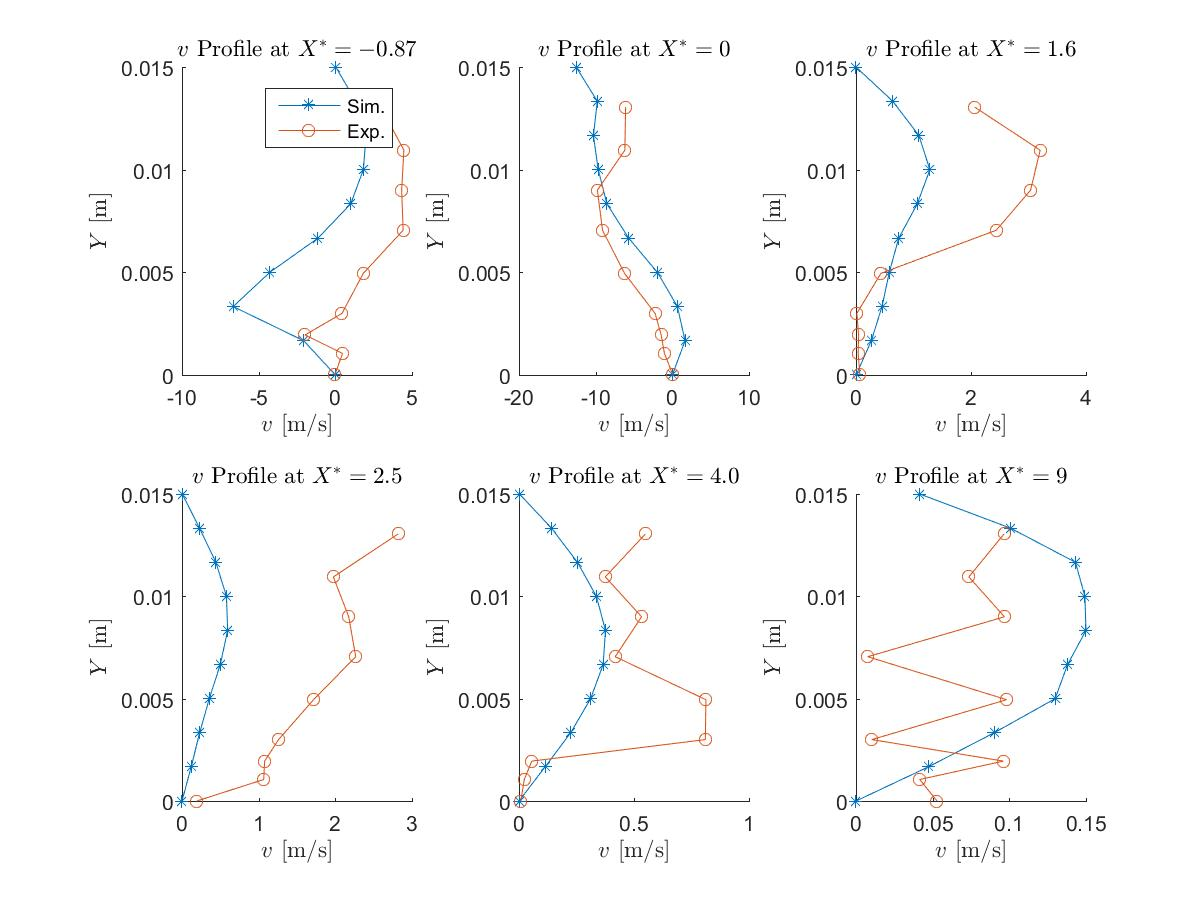
\includegraphics[scale=0.35]{matlab/exp_ref_v}
	\caption{Comparison of experimental and simulated $v$ profiles at various $X^*$.}
	\label{fig:exp_ref_v}
\end{figure}

Comments\\

Both simulated and experimental turbulent kinetic energy $k$ profiles at various $X^*$ are shown below in Figure~\ref{fig:exp_ref_k}.
\begin{figure}[H]
	\centering
	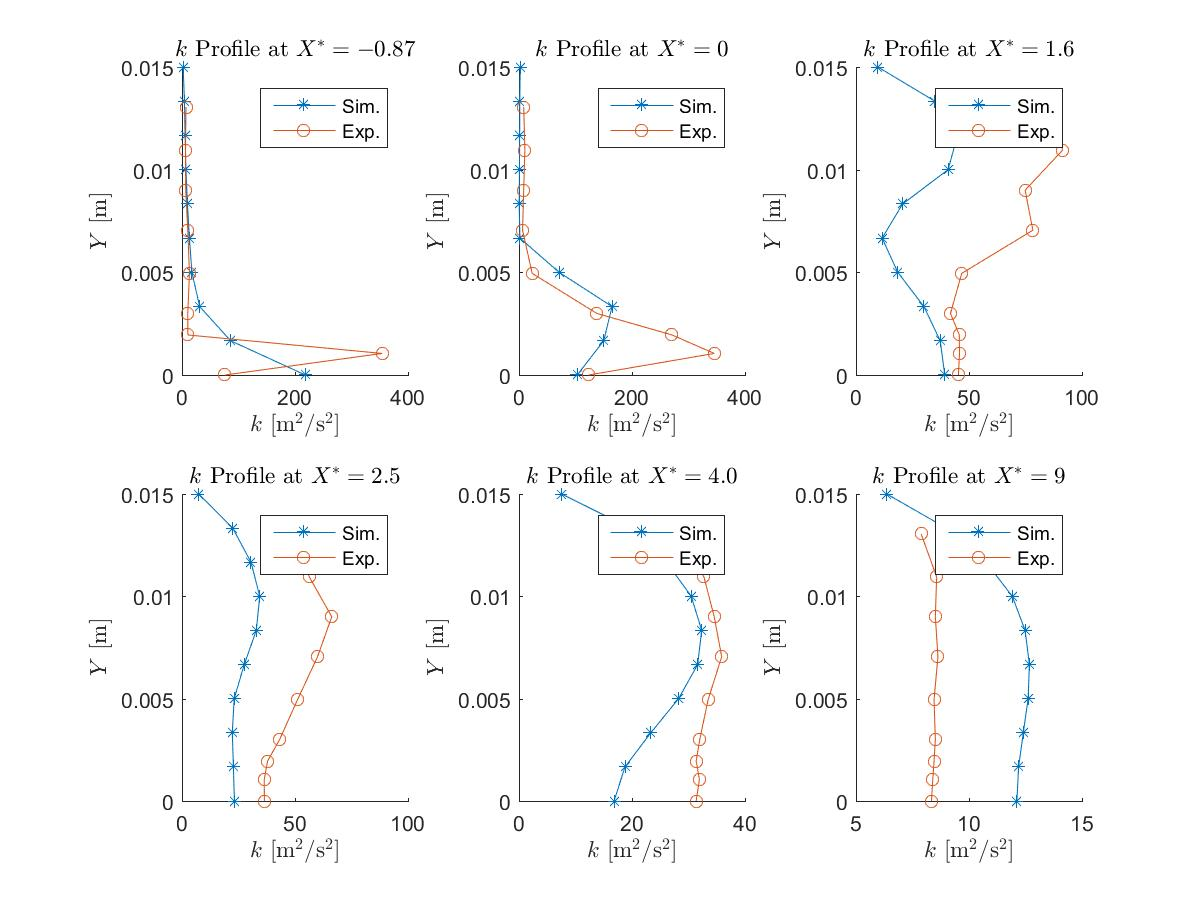
\includegraphics[scale=0.35]{matlab/exp_ref_k}
	\caption{Comparison of experimental and simulated $k$ profiles at various $X^*$.}
	\label{fig:exp_ref_k}
\end{figure}

Comments\\

%-----------------------------------------------------------------------------------------------------------------
\section{Effects of Side Inlets}
\label{sec:effects_side}

All simulated $u$ profiles at various $X^*$ are shown below in Figure~\ref{fig:sim_compu}.
\begin{figure}[H]
	\centering
	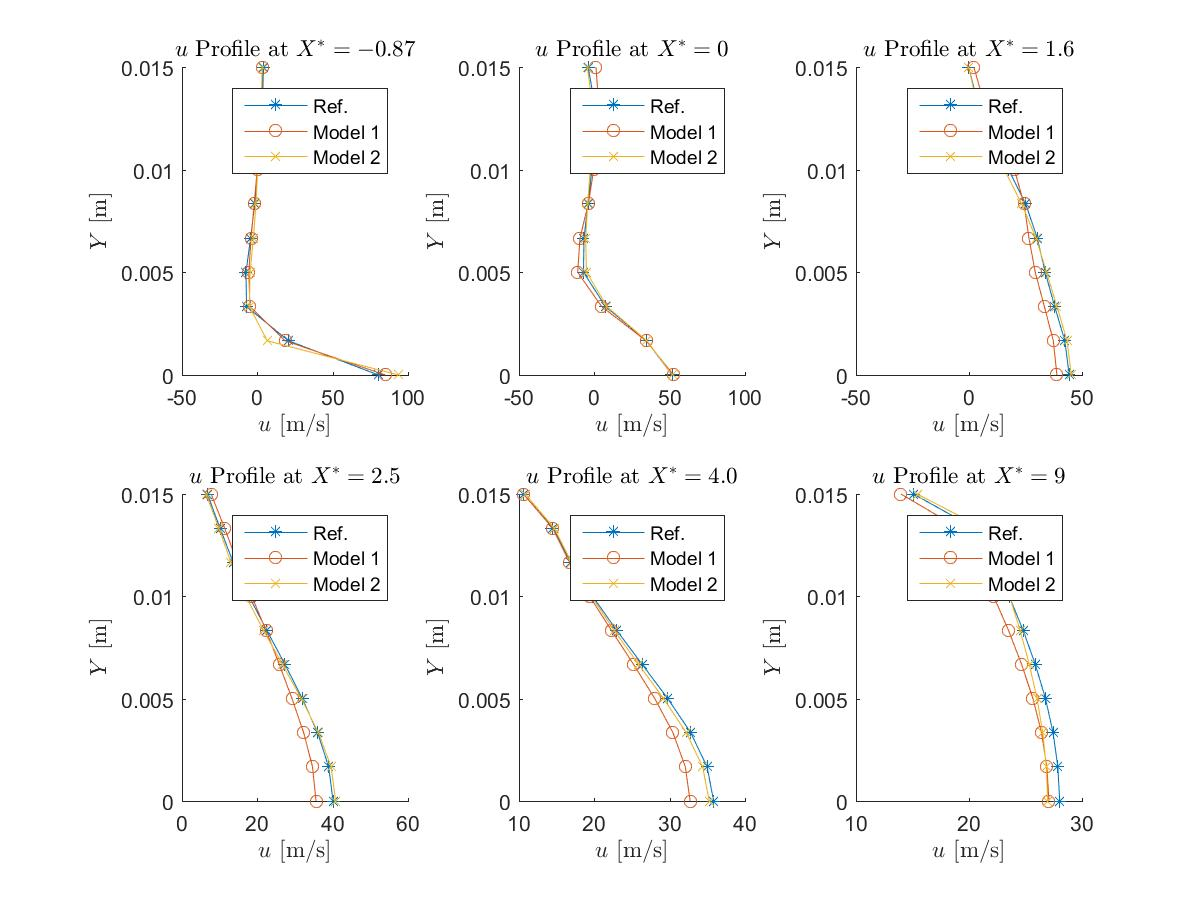
\includegraphics[scale=0.35]{matlab/sim_compu}
	\caption{Comparison of all simulated $u$ profiles at various $X^*$.}
	\label{fig:sim_compu}
\end{figure}


All simulated $v$ profiles at various $X^*$ are shown below in Figure~\ref{fig:sim_compu}.
\begin{figure}[H]
	\centering
	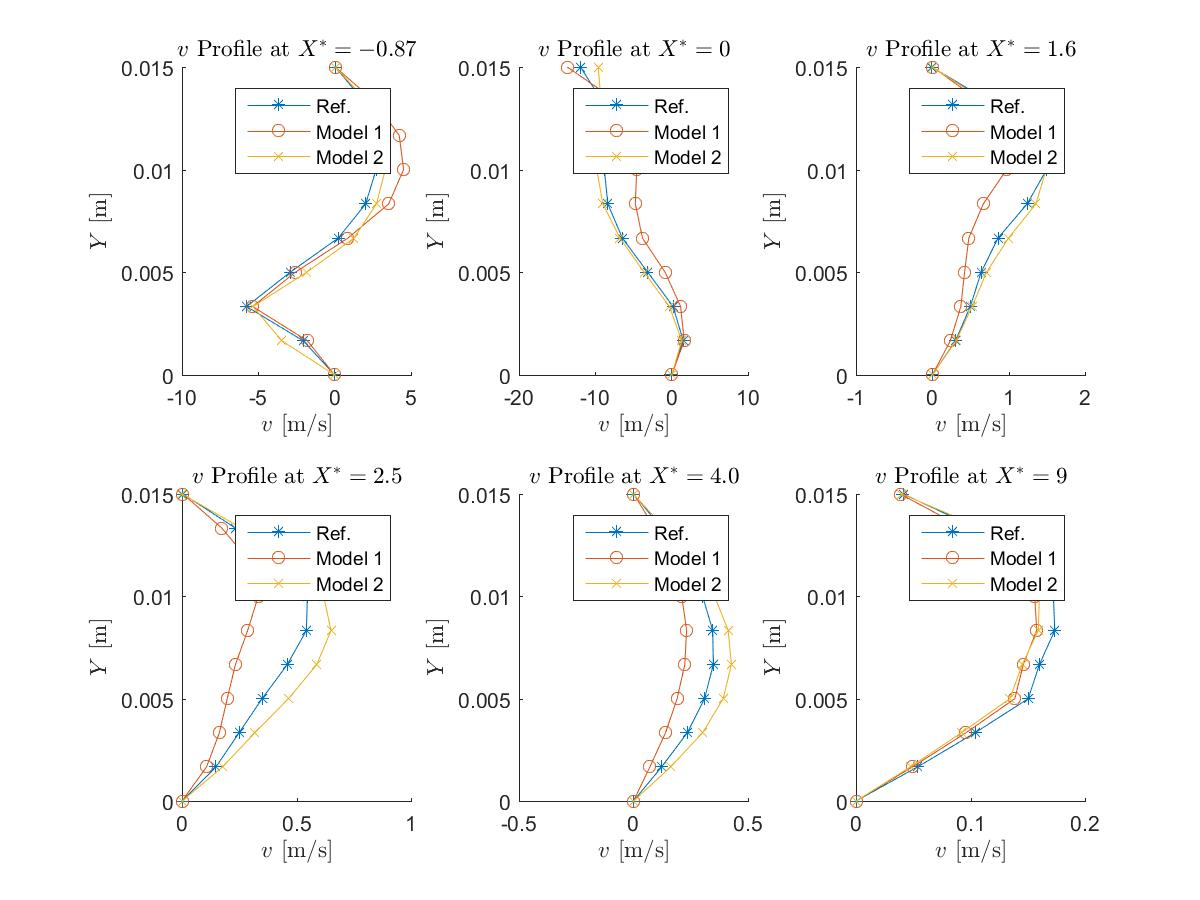
\includegraphics[scale=0.35]{matlab/sim_compv}
	\caption{Comparison of all simulated $v$ profiles at various $X^*$.}
	\label{fig:sim_compv}
\end{figure}


All simulated $k$ profiles at various $X^*$ are shown below in Figure~\ref{fig:sim_compk}.
\begin{figure}[H]
	\centering
	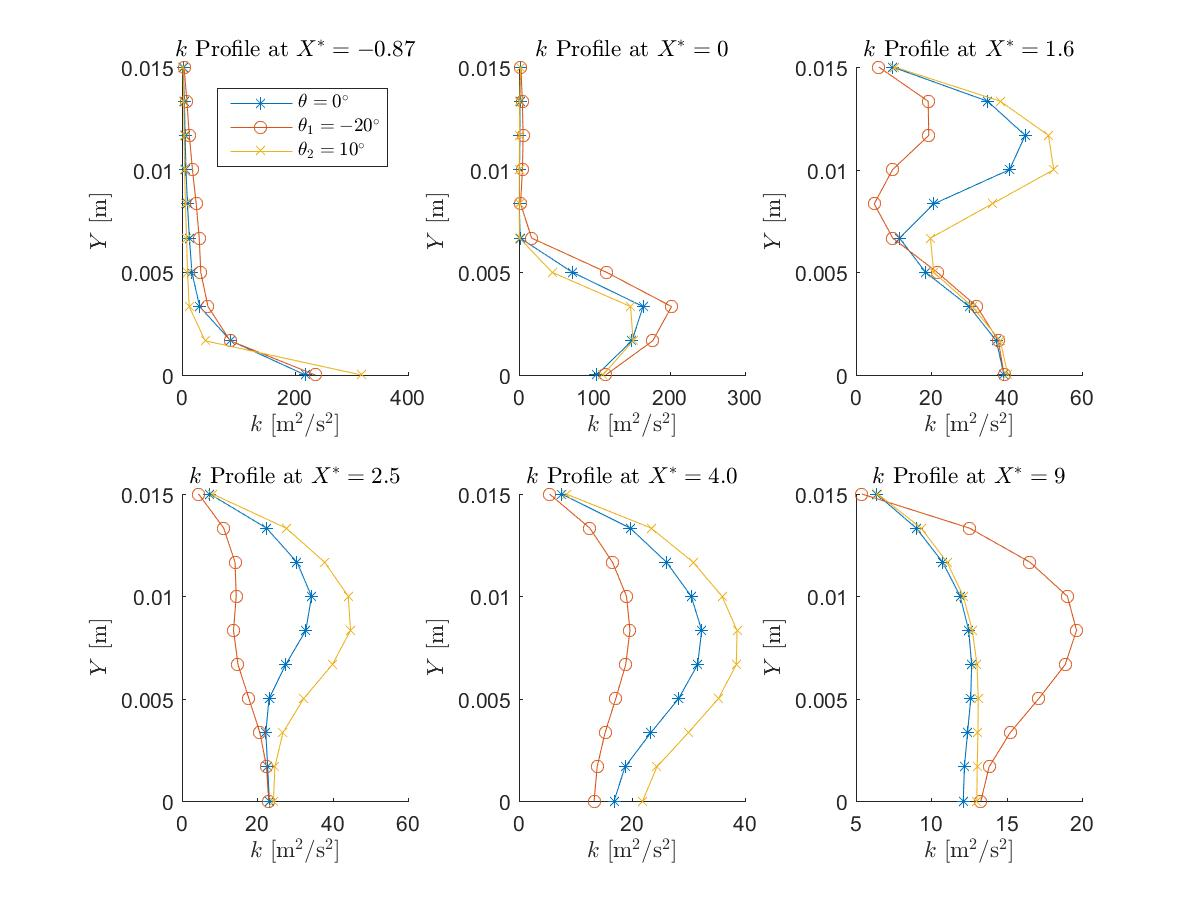
\includegraphics[scale=0.35]{matlab/sim_compk}
	\caption{Comparison of all simulated $k$ profiles at various $X^*$.}
	\label{fig:sim_compk}
\end{figure}

All simulated $T$ profiles at various $X^*$ are shown below in Figure~\ref{fig:sim_compT}.
\begin{figure}[H]
	\centering
	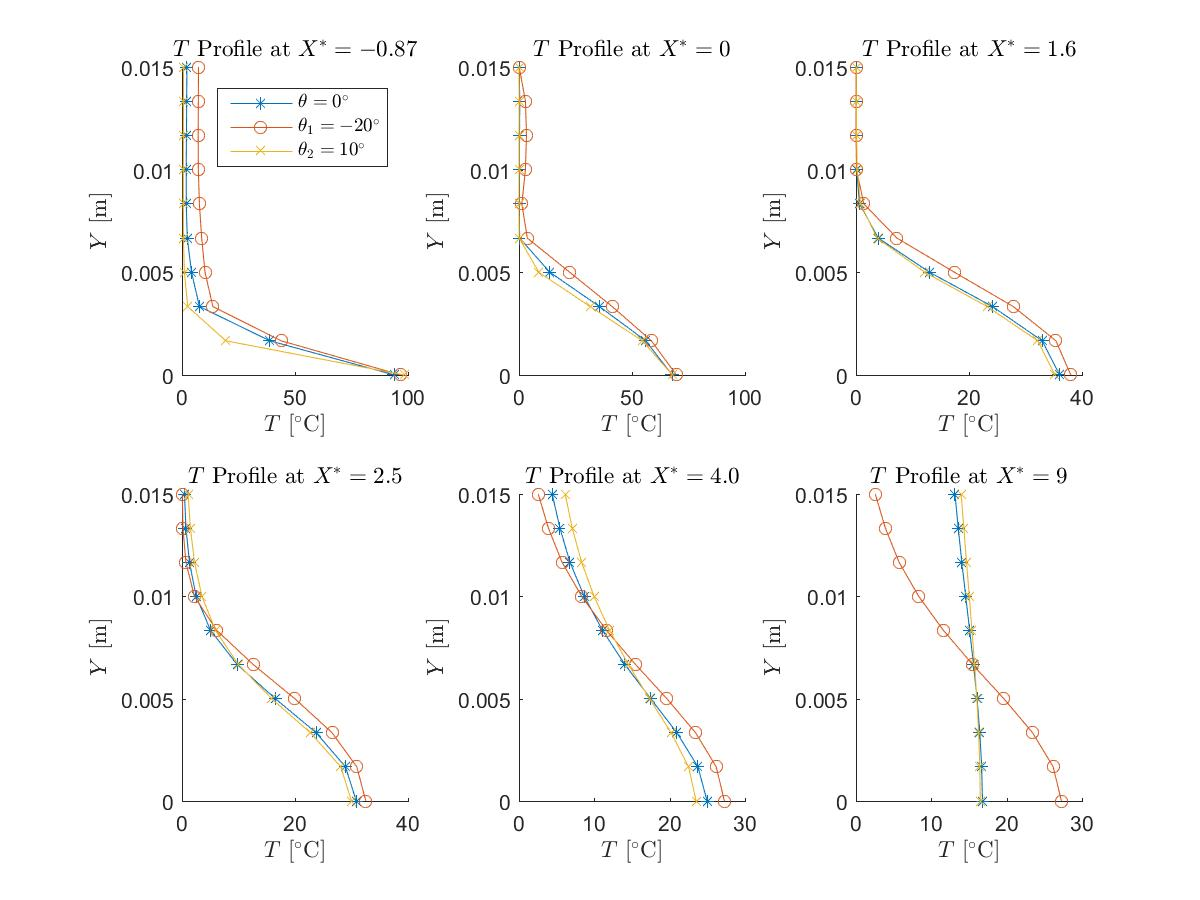
\includegraphics[scale=0.35]{matlab/sim_compT}
	\caption{Comparison of all simulated $T$ profiles at various $X^*$.}
	\label{fig:sim_compT}
\end{figure}


Variation of temperature $T$ along $X^*$ at $Y^*=0$ is shown below in Figure~\ref{fig:sim2_comp_T}.
\begin{figure}[H]
	\centering
	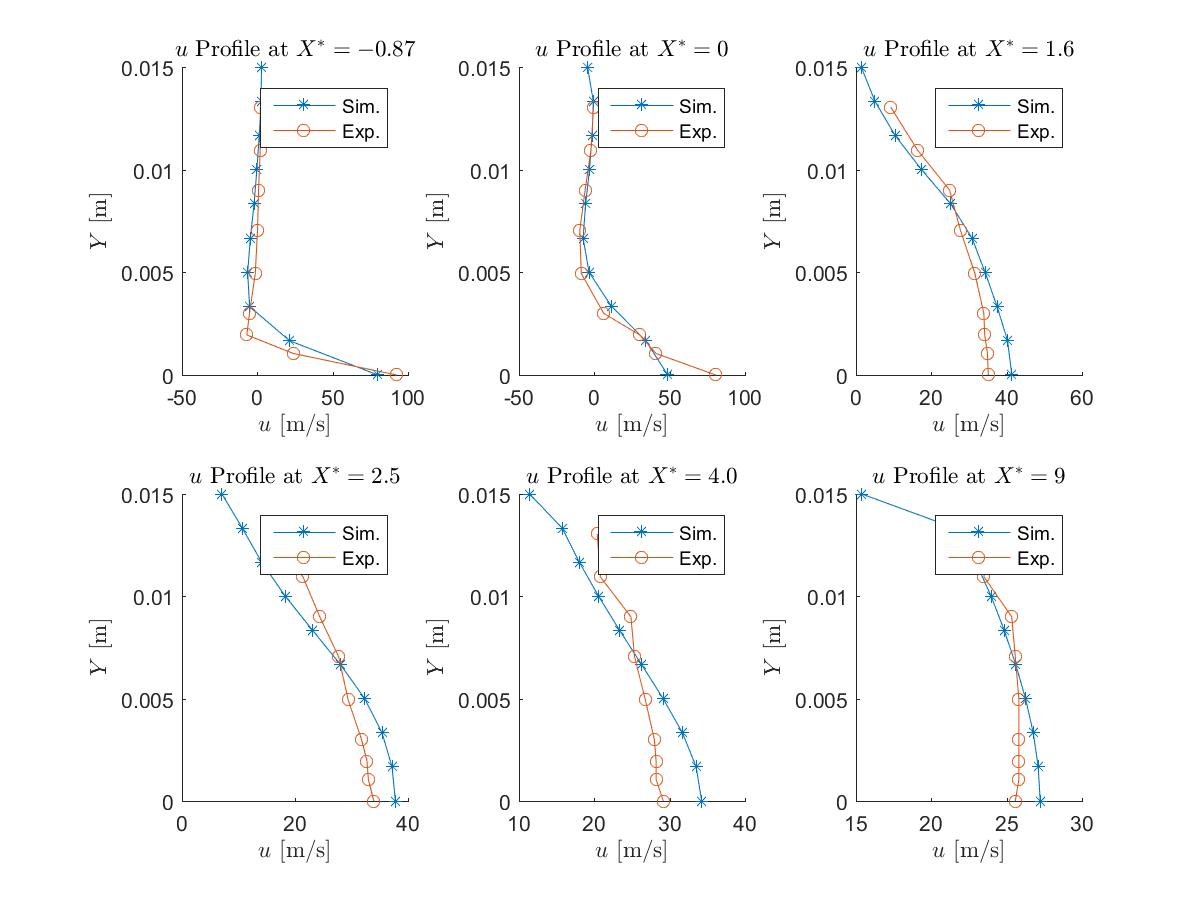
\includegraphics[scale=0.35]{matlab/sim2_comp_T}
	\caption{Variation of $T$ along $X^*$ at $Y^*=0$.}
	\label{fig:sim2_comp_T}
\end{figure}

Variation of velocity vector $\vec{V}$ along $X^*$ at $Y^*=0$ is shown below in Figure~\ref{fig:sim2_comp_V}.
\begin{figure}[H]
	\centering
	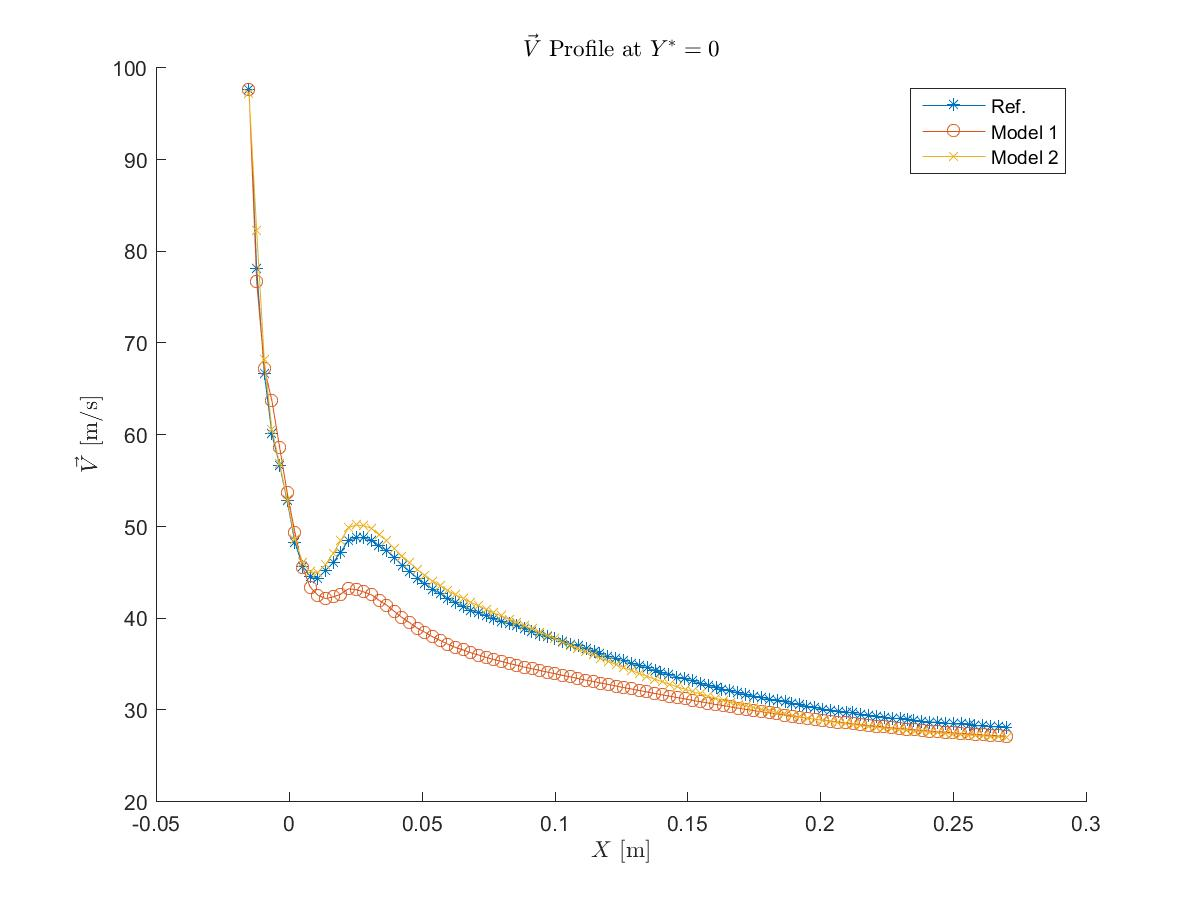
\includegraphics[scale=0.35]{matlab/sim2_comp_V}
	\caption{Variation of $\vec{V}$ along $X^*$ at $Y^*=0$.}
	\label{fig:sim2_comp_V}
\end{figure}


%-----------------------------------------------------------------------------------------------------------------
\section{Comparison}
\label{sec:comp}


%-----------------------------------------------------------------------------------------------------------------
\section{Source of Errors}
\label{sec:err}

